\documentclass[a4paper, 11pt]{article}
\usepackage[utf8]{inputenc}
\usepackage[polish]{babel}
\usepackage[MeX]{polski}
\usepackage[T1]{fontenc}
\usepackage{geometry}
\usepackage{fancyhdr}
\usepackage{graphicx}
\frenchspacing %wyłączenie dłuższych spacji na końcu każdego zdania.

\geometry{a4paper,tmargin=2.5 cm,bmargin=1.5cm,lmargin=2cm,rmargin=2cm}
\setlength{\headheight}{11pt} %przesuwa calosc w dol
\setlength{\headsep}{0.5cm} %przesuwa zawartosc wraz z dolna stopka w dol (bez gornej stopki
\setlength{\footskip}{1.2cm} %przesuwa w dol stopke od bmargin - konca tekstu

\newcommand{\przedmiot}{Indywidualny Projekt Programistyczny}
\newcommand{\podpisAutora}{Rafał Soszyński, nr indeksu 335786}
\newcommand{\data}{\today}%zamienić jeśli inaczej

\newcommand*{\naglowek}{
\begin{center}
{\huge \underline{\przedmiot}}
\\\vspace{0.50cm}
%% Koniecznie uzupełnić numer
Opis projektu: Gra planszowa typu RPG
\\\vspace{0.1cm}
{\large \textbf{\podpisAutora}}
\\\vspace{0.15cm}
\small{\data}
\\\vspace{1cm}
\end{center}
}

\begin{document}
\naglowek

\noindent\textbf{Zasady gry:}

Jest to gra typu RPG, gdzie każdy gracz posiada własną postać z określonymi statystykami i ekwipunkiem, którą rozwija przez całą rozgrywkę.
Gracz wybiera jaką klasą (np. łowca, mag) oraz klasą (np. elf, człowiek) będzie grał (ma to m.in. wpływ na statystykę oraz ekwipunek).
Gracze poruszają się systemem turowym po planszy złożonej z hexów.
Każde pole ma określony rodzaj (np. las, góra droga), co wpływa na możliwość wykonania ruchu.
Niektóre z pól są wyszczególnione i na nich odbywają się walki z przygotowanymi przeciwnikami.
Walka skłąda się z naprzemiennych ataków lub działań specjalnych (jak użycie przedmiotu).
Są też pola-miasta gdzie gracz może podjąć się jakiegoś zadania (typu przynieś, zbierz, zabij, itp.), handlować ekwipunkiem czy uleczyć swoją postać.
Na wspomniany ekwipunek składają się pancerz, broń, mikstury oraz artefakty.
Gra kończy się w przypadku, gdy jeden z graczy osiągnie określony poziom i wykona pewne trudne zadanie (ze specjalnej puli).

\vspace{0,5cm}

\noindent\textbf{Opis modułów programu:}

\begin{itemize}
	\item \underline{Okno Nowej Gry}: Wyświetla okno pozwalające wprowadzić ustawienia początkowe rozgrywki.
	
	\item \underline{Cykl Gry}: Zarządza przebiegiem gry. Określa aktualnego gracza oraz moment gry.
	
	\item \underline{Plansza}: Trzyma informacje o układzie planszy, udostępnia listę możliwych ruchów dla gracza.
	
	\item \underline{Parser Układu}: Pobiera z dysku ustawienie planszy.
	
	\item \underline{Obszar Planszy}: Odpowiada za wyświetlanie hexów na ekranie i wodotryski. Udostępnia wyświetlenie konkretnego ruchu gracza.
	
	\item \underline{Mistrz Gry}: Odpowiada za wyznaczanie możliwych akcji gracza oraz nadzorowanie walk. Dodatkowo prosi o wyświetlenie komponenty graficzne (poza Obszarem Planszy, za który odpowiada Plansza), a także w razie potrzeby odbiera od nich "wyklikane" informacje. Udostępnia informacje o graczu.
	
	\item \underline{ParserKart}: Pobiera z dysku bazę zadań, przedmiotów i przeciwników oraz przekazuje ją Mistrzowi Gry.
	
	\item \underline{Panel Akcji}: Wyświetla na rządanie listę akcji i informuje o ewentualnym wyborze.
	
	\item \underline{Okno Gracza}: Wyświetla obecne dane gracza. Pozwala na wyświetlenie Ekwipunku i Zadań.
	
	\item \underline{Ekwipunek}: Wyświetla i pozwala zarządzać ekwipunkiem gracza.
	
	\item \underline{Zadania}: Wyświetla i pozwala zarządzać podjętymi zadaniami gracza. 
	
	\item \underline{Tawerna}: Wyświetla okno tawerny (miejsca w mieście, gdzie gracz może podjąć się nowych zadań).

	\item \underline{Bazar}: Wyświetla okno bazaru (miejsca w mieście, gdzie gracz może handlować ekwipunkiem).

	\item \underline{Walka}: Wyświetla okno walki.

	\item \underline{AI}: Jako implementacja sztucznej inteligencji udostępnia podejmowanie decyzji o ruchu na podstawie dostępnych akcji. Ma do dyspozycji listę pól udestępnianą przez Planszę oraz dane od Mistrza Gry.
\end{itemize}

\newpage

\begin{figure}[ht]

\centering

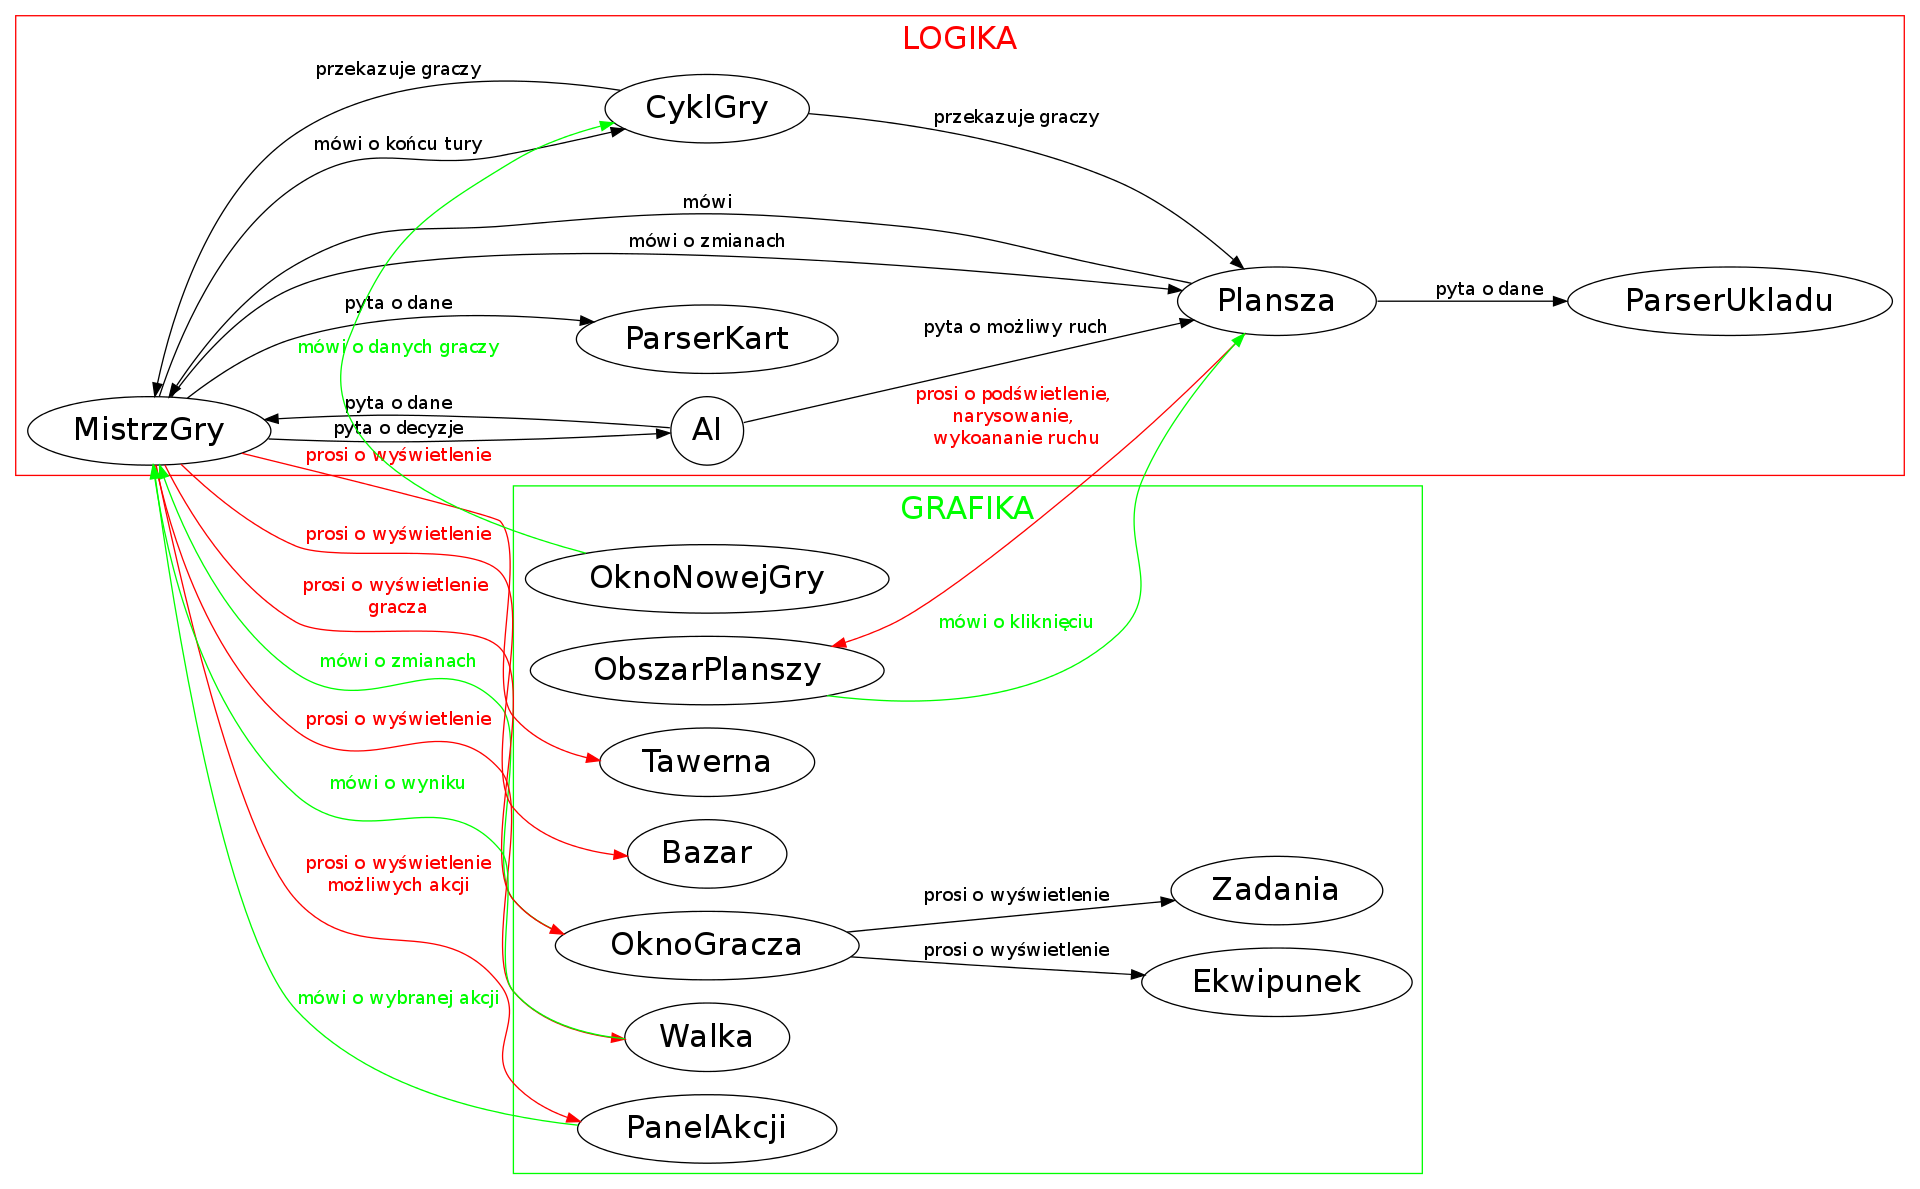
\includegraphics[scale=0.24]{klasy.png}

\caption{Graf modułów projektu z uwzględnieniem podziału na warstwę graficzną i logiczną.} 

\label{Klasy}

\end{figure}

\noindent\textbf{Możliwe rasy w grze:} \textit{Człowiek, Krasnolud, Elf, Niziołek}

\noindent\textbf{Możliwe klasy w grze:} \textit{Wojownik, Łowca, Mag, Druid }

\vspace{0.5cm}
\noindent\textbf{Postać plików na dysku:}

\textbf{Format zapisu przedmiotów:}

Każdy przedmiot zapisany jest w oddzielnej linii. \underline{Kolejność informacji:}

\textit{identyfikator;nazwa przedmiotu;typ;bonus do walki wrecz;b.d.w. dystansowej;b.d.w. magicznej; modyfikator obrony;m. percepcji; m. zdrowia;m. regeneracji ;ograniczenie względem klasy;czy bron jednoreczna;czy dostępna od 5 poziomu;wartość;kolor czcionki;
}

Ograniczenia względem klas podawane są w tej kolejności: wojownik, łowca, mag, druid\\ (1 może , 0 nie może nosić) np. 1010.

\underline{Typy przedmiotow} (odpowiadające miejscu założenia): 
\begin{itemize}
	\item w - bron (prawa reka)
	\item t - tarcza lub aura (nie można łączyć z bronią dwuręczną)
	\item p - pancerz lekki 
	\item h - hełm
	\item a - artefakt
	\item m - mikstura
\end{itemize}

\underline{Możliwe kolory czcionki:} b-biały, n-niebieski, c-czerwony.

Przedmioty przynależą do grup. Linie postaci $ \$nazwaGrupy $ rozpoczynają przypisywanie przedmiotów do danej grupy. Przypisane zostają do niej wszystkie przedmioty, aż do końca pliku lub zdefiniowania kolejnej grupy.
\begin{verbatim}
Przykład:
$M1B
3;DOBRY MIECZ;w;1;0;0;0;0;0;0;1100;1;0;1;b
4;WYWAŻONY MIECZ;w;2;0;0;0;0;0;0;1100;1;0;1;b
\end{verbatim}
\textbf{Format zapisu nagród:}

Każda nagroda zapisana jest w oddzielnej linii. \underline{Kolejność informacji:}

\textit{identyfikator;zmiana reputacji(ludzie, krasnoludy, elfy, niziołki);złoto;doświadczenie;grupa z której losowany jest przedmiot; ID konkretnego przedmiotu}

\underline{Format:}
liczba całkowita;4 l. całkowite oddzielone przecinkami;l. całkowita;l. całkowita, tekst, l. całkowita
\begin{verbatim}
Przykład:
1;1,0,0,1;5;200;AN;
2;0,0,0,-1;2;100;;122
3;0,0,2,0;5;300;;
\end{verbatim}

\noindent\textbf{Format zapisów zadań:}

Każde zadanie zapisane jest w oddzielnej linii. \underline{Kolejność informacji:}

\textit{identyfikator;typ zadania; tytuł; treść; czy powrót wymagany; kolor czcionki; pole celu;id nagrody; lista przeciwników}

\underline{Format:}
liczba całkowita;tekst; tekst;0 albo 1; znak; 2 l. całkowite oddzielone przecinikiem; l. całkowita; liczby całkowite oddzielone przecinkami

\underline{Typy zadań:} 
\begin{itemize}
	\item 1 - Idź i pokonaj przeciwnika(ów)
	\item 2 - Idź gdzieś / Zbierz kilka przedmiotów
	\item 3 - Odnajdź kogoś (dotrzyj na pole i rzuć kością czy się udało)
\end{itemize}

\underline{Możliwe kolory czcionki:} b-biały, n-niebieski, c-czerwony.

\begin{verbatim}
Przykład:
1;Potrzebne lekarstwo;Młody chłopak z wioski został ukąszony przez żądlika. Jedynym
lekarstwem jest mikstura z dodatkiem jadu. Mama chłopca prosi cię o zebranie 2 żądeł.
Żądliki znajdziesz nieopodal lasu na polu 30,17.;1;b;30,17;1;4,4
2;Pastuszkowie, przybywajcie;Chłop prosi cię, abyś sprawdził, co atakuje bydło
pasące się na łące. Będziesz musiał pokonać młodego wilka niepokojącego stado.
Udaj się na pole 21,2;0;z;21,2;90;3
3;Bunt;Kilku żołnierzy zbuntowało się przeciw swojemu dowódcy. Pokonaj przywódcę
buntu na polu 11,15.;0;c;11,15;3;45
\end{verbatim}

\noindent\textbf{Format zapisu przeciwników:}

Każdy przeciwnik zapisany jest w oddzielnej linii. \underline{Kolejność informacji:}

\textit{identyfikator; nazwa; nazwa pliku ze zdjęciem; opis; atak; obrona; zdrowie; id nagrody}

\underline{Format:}
liczba całkowita;tekst; tekst; tekst; l. całkowita; l. całkowita l. całkowita; l. całkowita

Atak jest reprezentowany jako dwie liczby całkowite stanowiące granice przedziału z którego losowana jest wartość.

\begin{verbatim}
Przykład:
1;Smok Spiro;smok5.jpg;Jeden z pięciu potężnych smoków i najtrudniejszych 
przeciwników w całej krainie.;40,46;48;30;2
2;Goblin zwiadowca;goblin1.png;Zwiadowca niedużej grupy goblinów ukrywającej
się w lasach.;8,12;16;10;1
3;Szkielet niszczyciel;szkiel3.jpg;Mocna, zaprawiona w boju jednostka bojowa
nieumarłych.;20,25;30;22;3
\end{verbatim}

\newpage

\textbf{Format zapisu planszy:}
\begin{verbatim}
szerokość;wysokość           (2 liczby całkowite dodatnie)

liczba wpisów w legendzie    (liczba całkowite dodatnie)

symbol; nazwa; plik z obrazkiem; czy jest przeciwnik; współczynnik ruchu 
    Format linii legendy:    (tekst(bez spacji);tekst;tekst;1 lub 0; liczba całkowita)

Następnie znajduje się tyle wierszy ile plansza ma wysokości, 
zawierające tyle pól ile szerokości ma plansza.
Pola poodzielane są średnikami i zawierają symbole pól na odpowiednich pozycjach

\end{verbatim}

\begin{figure}[ht]

\centering

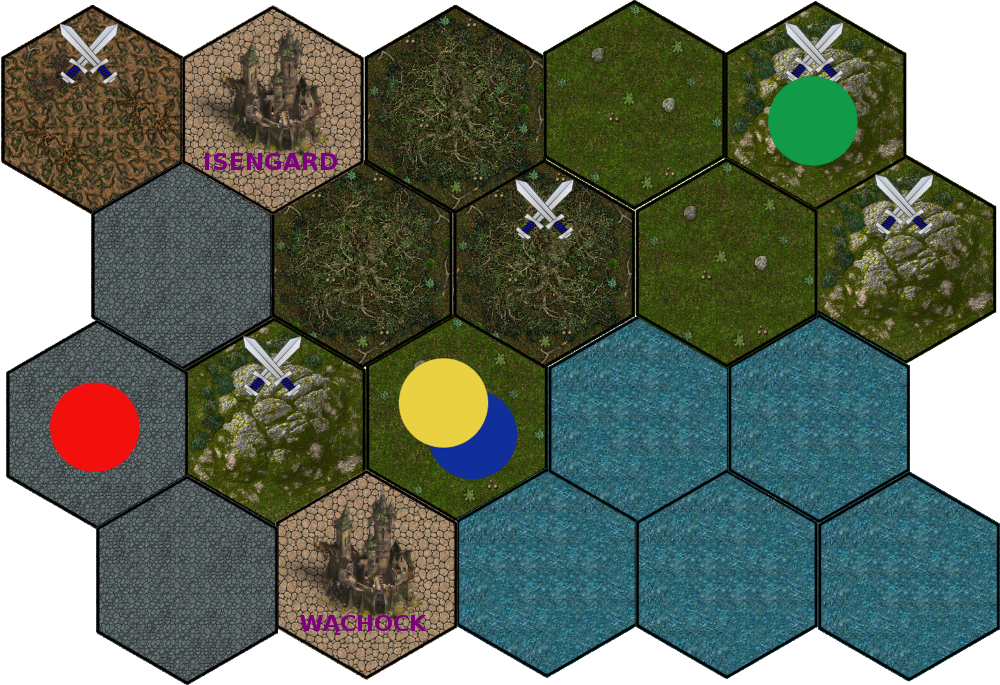
\includegraphics[scale=0.3]{plansza.png}

\caption{Przykładowa plansza.} 

\label{Klasy}

\end{figure}

Zawartość pliku z ustawieniem dla powyższej planszy
\begin{verbatim}
5;4
9
B;;bagno.png;1;3
1;ISENGARD;zamek.png;0;0
l;;las.png;0;2
L;;las.png;1;2
d;;dolina.png;0;1
G;;gora.png;1;2
a;;droga.png;0;1
2;WĄCHOCK;zamek.png;0;0
w;;woda.png;0;2
B;1;l;d;G
 a;l;l;d;G
a;G;d;w;w
 a;2;w;w;w	
\end{verbatim}

\end{document}
